
\documentclass[aspectratio=169]{beamer}

% --- Theme / packages ---
% -------------------------------------------------
% Packages
% -------------------------------------------------
\usepackage{amsmath, amsfonts}
\usepackage{graphicx}
\usepackage{booktabs}
\usepackage{hyperref}
\usepackage{bm}
\usepackage{siunitx}
\usepackage{listings}

% Figure search paths (relative to tex/lectures/)
\graphicspath{{../figures/lectures/}{../figures/shared/}}

% -------------------------------------------------
% Notes (speaker notes)
% -------------------------------------------------
\usepackage{pgfpages}
% Uncomment ONE of these for speaker notes:
% \setbeameroption{show notes} % notes only (for printing notes)
% \setbeameroption{show notes on second screen=right} % slides + notes

% -------------------------------------------------
% TikZ
% -------------------------------------------------
\usepackage{tikz}
\usetikzlibrary{matrix, calc}
\usepackage{xcolor} % (tikz loads xcolor, but explicit is fine)
\usetikzlibrary{arrows.meta, decorations.pathreplacing}


% -------------------------------------------------
% Themes
%--------------------------------------------------
\usetheme{default}
\usecolortheme{default}
\setbeamertemplate{navigation symbols}{}

% -----------------------------
% Code formatting
% -----------------------------
\definecolor{codegray}{RGB}{245,245,245}

\lstset{
  backgroundcolor=\color{codegray},
  basicstyle=\ttfamily\small,
  frame=single,
  breaklines=true,
  showstringspaces=false
}

% --- Shortcuts ---
%\newcommand{\dd}{\,\mathrm{d}}
\newcommand{\Grad}{\nabla}
\newcommand{\Div}{\nabla\!\cdot}
\newcommand{\bx}{\bm{x}}
\newcommand{\bn}{\bm{n}}
\newcommand{\bq}{\bm{q}}

%==========================
% Flipbook macro (put in preamble or before frames)
%==========================
\newcommand{\GSFlipFrame}[2]{%
\begin{frame}{Gauss--Seidel sweep (current point $(#1,#2)$)}
\centering
\hspace{3.5cm}
\vspace{3cm}
\begin{tikzpicture}[scale=2.2, every node/.style={font=\small}]
  % -----------------------------
  % USER SETTINGS
  % -----------------------------
  \def\Nx{6}   % i = 0..Nx-1
  \def\Ny{4}   % j = 0..Ny-1

  % current stencil location (interior)
  \def\ci{#1}
  \def\cj{#2}

  % Point spacing
  \def\s{0.85}

  % -----------------------------
  % STYLES
  % -----------------------------
  \tikzset{
    gpG/.style={circle, fill=green!70!black, inner sep=1.1pt},
    gpR/.style={circle, fill=red!75!black,   inner sep=1.1pt},
    gpbG/.style={circle, fill=green!70!black, inner sep=1.5pt},
    gpbR/.style={circle, fill=red!75!black,   inner sep=1.5pt},
    gpc/.style={circle, fill=blue, inner sep=1.7pt},
    stline/.style={dashed, thick},
    labij/.style={font=\normalsize},
    labp/.style={font=\scriptsize, text=gray!70},
  }

  % -----------------------------
  % OUTER RECTANGLE (domain)
  % -----------------------------
  \draw[thick] (0,0) rectangle ({(\Nx-1)*\s},{(\Ny-1)*\s});

  % -----------------------------
  % GRID POINTS + LABELS
  % -----------------------------
  \foreach \j in {0,...,\numexpr\Ny-1\relax} {
    \foreach \i in {0,...,\numexpr\Nx-1\relax} {

      \pgfmathsetmacro{\x}{\i*\s}
      \pgfmathsetmacro{\y}{\j*\s}

      % global index p = i + j*Nx (as in your first figure)
      \pgfmathtruncatemacro{\p}{\i + \j*\Nx}

      % boundary?
      \pgfmathtruncatemacro{\isB}{ (\i==0) || (\i==\Nx-1) || (\j==0) || (\j==\Ny-1) }
      % current center?
      \pgfmathtruncatemacro{\isC}{ (\i==\ci) && (\j==\cj) }

      % "already updated" (GS ordering): j<cj OR (j==cj and i<ci)
      \pgfmathtruncatemacro{\isUpdated}{ (\j<\cj) || ((\j==\cj) && (\i<\ci)) }

      % FORCE left boundary (i==0) and bottom boundary (j==0) to be green
      \pgfmathtruncatemacro{\forceGreen}{ \isB }

      % decide color state:
      % - center: blue
      % - else green if forced green OR updated
      % - else red
      \ifnum\isC=1
        \node[gpc] (P\i\j) at (\x,\y) {};
      \else
        \pgfmathtruncatemacro{\isGreen}{ (\forceGreen==1) || (\isUpdated==1) }
        \ifnum\isB=1
          \ifnum\isGreen=1
            \node[gpbG] (P\i\j) at (\x,\y) {};
          \else
            \node[gpbR] (P\i\j) at (\x,\y) {};
          \fi
        \else
          \ifnum\isGreen=1
            \node[gpG] (P\i\j) at (\x,\y) {};
          \else
            \node[gpR] (P\i\j) at (\x,\y) {};
          \fi
        \fi
      \fi

      % Labels (i,j) above-right; p below-right
      \node[labij, anchor=south west] at (\x+0.05,\y+0.05) {$(\i,\j)$};
      \node[labp,  anchor=north west] at (\x+0.05,\y-0.05) {$\p$};
    }
  }

  % -----------------------------
  % 5-POINT STENCIL (dashed)
  % -----------------------------
  \pgfmathsetmacro{\xc}{\ci*\s}
  \pgfmathsetmacro{\yc}{\cj*\s}

  \draw[stline] (\xc,\yc) -- ({(\ci+1)*\s},\yc);
  \draw[stline] (\xc,\yc) -- ({(\ci-1)*\s},\yc);
  \draw[stline] (\xc,\yc) -- (\xc,{(\cj+1)*\s});
  \draw[stline] (\xc,\yc) -- (\xc,{(\cj-1)*\s});

  % Mapping note
  %\node[font=\scriptsize, align=left] at ({(1)*\s+1.65},{(0)*\s-0.55})
  %{$p = i + j\,N_x$};
\end{tikzpicture}
\end{frame}%
}













%-------------------------------------------------
% Title information
%-------------------------------------------------
\title{Two-Dimensional Heat Conduction}
\subtitle{Finite Differences and the Five-Point Stencil}
\author{MMAE 450: Computational Mechanics II}
\date{}

%=================================================
\begin{document}

%-------------------------------------------------
\begin{frame}
  \titlepage
\end{frame}

%=================================================
\begin{frame}{Motivation for 2D Heat Conduction}
\begin{itemize}
  \item Many engineering problems involve temperature variation in more than one spatial direction.
  \item Examples:
  \begin{itemize}
    \item Thin plates and heat sinks
    \item Cooling of electronic components
    \item Layered or composite materials
  \end{itemize}
  \item Extending 1D ideas to 2D is conceptually straightforward.
  \item The resulting algebraic systems become \emph{large} and \emph{sparse}.
\end{itemize}
\end{frame}

%=================================================
\begin{frame}{Governing Equation in Two Dimensions}
For a homogeneous, isotropic material with constant properties:
\vspace{0.5em}
\begin{equation*}
\frac{\partial T}{\partial t}
=
\alpha\left(
\frac{\partial^2 T}{\partial x^2}
+
\frac{\partial^2 T}{\partial y^2}
\right)
\end{equation*}
\vspace{0.5em}
Under steady-state conditions:
\begin{equation*}
\frac{\partial^2 T}{\partial x^2}
+
\frac{\partial^2 T}{\partial y^2}
= 0
\end{equation*}
\vspace{0.5em}
\begin{itemize}
  \item This is the 2D \emph{Laplace equation}.
  \item Boundary conditions (Dirichlet/Neumann/Robin) are prescribed on $\partial\Omega$.
\end{itemize}
\end{frame}

%=================================================
\begin{frame}{Rectangular Domain and Grid}
Consider a rectangular plate:
\begin{itemize}
  \item $0 \le x \le L_x$
  \item $0 \le y \le L_y$
\end{itemize}
\vspace{0.5em}
Uniform grid:
\begin{equation*}
\Delta x = \frac{L_x}{N_x-1}, \qquad
\Delta y = \frac{L_y}{N_y-1}
\end{equation*}
\vspace{0.5em}
Grid points labeled by $(i,j)$:
\begin{align*}
 x_i &= i\,\Delta x, \quad i=0,1,\dots,N_x,\\
 y_j &= j\,\Delta y, \quad j=0,1,\dots,N_y.
\end{align*}
We denote the nodal approximation by $T_{i,\,j}^n \approx T(x_i,y_j,t^n)$.
\end{frame}

%=================================================
\begin{frame}{Five-Point Stencil}
\centering
\includegraphics[width=0.85\textwidth]{../figures/lectures/chap03_fig10_rect-stencil.png}
\vspace{0.5em}
\begin{itemize}
  \item Interior node $(i,j)$ depends on four nearest neighbors.
  \item This produces the classic \emph{five-point stencil}.
\end{itemize}
\end{frame}

%=================================================
\begin{frame}{Discrete Laplacian}
Second derivatives using centered finite differences:
\begin{align*}
\left.\frac{\partial^2 T}{\partial x^2}\right|_{i,\,j}
&\approx
\frac{T_{i+1,\,j} - 2T_{i,\,j} + T_{i-1,\,j}}{(\Delta x)^2}, \\
\left.\frac{\partial^2 T}{\partial y^2}\right|_{i,\,j}
&\approx
\frac{T_{i,\,j+1} - 2T_{i,\,j} + T_{i,\,j-1}}{(\Delta y)^2}.
\end{align*}
\vspace{0.5em}
If $\Delta x = \Delta y = h$, then
\begin{equation*}
\nabla^2 T\big|_{i,\,j}
\approx
\frac{T_{i+1,\,j}+T_{i-1,\,j}+T_{i,\,j+1}+T_{i,\,j-1}-4T_{i,\,j}}{h^2}.
\end{equation*}
\end{frame}

%=================================================
\begin{frame}{Steady-State as a Linear System}
At each interior node, the discrete Laplace equation gives
\begin{equation*}
T_{i+1,\,j} + T_{i-1,\,j} + T_{i,\,j+1} + T_{i,\,j-1} - 4T_{i,\,j} = 0.
\end{equation*}
\vspace{0.5em}
Collecting all interior equations yields
\begin{equation*}
\mathbf{A}\,\mathbf{T} = \mathbf{d},
\end{equation*}
where
\begin{itemize}
  \item $\mathbf{T}$ contains the unknown interior temperatures,
  \item $\mathbf{A}$ is sparse (\emph{at most five nonzeros per row}),
  \item $\mathbf{d}$ accounts for prescribed boundary values.
\end{itemize}
\end{frame}

%=================================================
%=================================================
\begin{frame}{Structure of the Discrete System Matrix $\mathbf{A}$}

For the five-point stencil, the steady problem
\[
\mathbf{A}\,\mathbf{T} = \mathbf{d}
\]
leads to a sparse matrix with a highly regular structure.

\vspace{0.5em}

\centering
\begin{equation*}
\mathbf{A} =
\begin{bmatrix}
\ddots & \ddots &        &        &        \\
\ddots & -4     &  1     &        &        \\
       &  1     & -4     &  1     &        \\
       &        &  1     & -4     & \ddots \\
       &        &        & \ddots & \ddots
\end{bmatrix}
\end{equation*}

\vspace{0.5em}

\begin{itemize}
  \item Each row corresponds to one interior grid node
  \item Diagonal entry ($-4$): contribution from $T_{i,\,j}$
  \item Off-diagonals ($+1$): coupling to nearest neighbors
  \item Overall structure is sparse and banded
\end{itemize}

\end{frame}
%============================
\begin{frame}
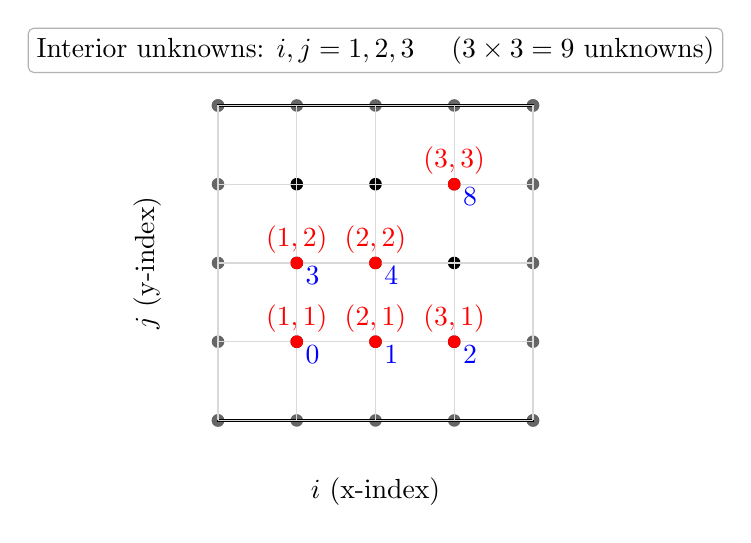
\begin{tikzpicture}[x=1.0cm,y=1.0cm,>=latex]

% ------------------------------------------------------------
% Draw all grid nodes (5x5): i,j = 0..4
% ------------------------------------------------------------
\foreach \j in {0,...,4} {
  \foreach \i in {0,...,4} {
    \fill[black!30] (\i,\j) circle (0.06);
  }
}

% ------------------------------------------------------------
% Emphasize boundary nodes (Dirichlet)
% ------------------------------------------------------------
\foreach \i in {0,...,4} {
  \fill[black!60] (\i,0) circle (0.08);
  \fill[black!60] (\i,4) circle (0.08);
}
\foreach \j in {0,...,4} {
  \fill[black!60] (0,\j) circle (0.08);
  \fill[black!60] (4,\j) circle (0.08);
}

% ------------------------------------------------------------
% Emphasize interior nodes (unknowns): i,j = 1..3
% ------------------------------------------------------------
\foreach \j in {1,...,3} {
  \foreach \i in {1,...,3} {
    \fill[black] (\i,\j) circle (0.08);
  }
}

% Draw domain outline
\draw[thick] (0,0) rectangle (4,4);

% Light grid lines
\draw[black!15, step=1] (0,0) grid (4,4);

% ------------------------------------------------------------
% Label a few interior nodes with (i,j) and idx
% idx(i,j) = (j-1)*3 + (i-1)
% ------------------------------------------------------------

% (1,1) -> idx = 0
\fill[red] (1,1) circle (0.08);
\node[anchor=south, red] at (1.0,1.0)
{$(1,1)$};
\node[anchor=south, blue] at (1.2,0.6)
{$0$};

% (2,1) -> idx = 1
\fill[red] (2,1) circle (0.08);
\node[anchor=south, red] at (2.0,1.0)
{$(2,1)$};
\node[anchor=south, blue] at (2.2,0.6)
{$1$};

% (3,1) -> idx = 2
\fill[red] (3,1) circle (0.08);
\node[anchor=south, red] at (3.0,1.0)
{$(3,1)$};
\node[anchor=south, blue] at (3.2,0.6)
{$2$};

% (1,2) -> idx = 3
\fill[red] (1,2) circle (0.08);
\node[anchor=south, red] at (1.0,2.0)
{$(1,2)$};
\node[anchor=south, blue] at (1.2,1.6)
{$3$};

% (2,2) -> idx = 4
\fill[red] (1.999,2) circle (0.08);
\node[anchor=south, red] at (2.0,2.0)
{$(2,2)$};
\node[anchor=south, blue] at (2.2,1.6)
{$4$};

% (3,3) -> idx = 8
\fill[red] (3,3) circle (0.08);
\node[anchor=south, red] at (3.0,3.0)
{$(3,3)$};
\node[anchor=south, blue] at (3.2,2.6)
{$8$};

% ------------------------------------------------------------
% Axis annotations
% ------------------------------------------------------------
\node[anchor=north] at (2,-0.6) {$i$ (x-index)};
\node[anchor=south, rotate=90] at (-0.6,2) {$j$ (y-index)};

% Interior note
\node[fill=white, draw=black!30, rounded corners=2pt, inner sep=3pt]
at (2,4.7)
{Interior unknowns: $i,j=1,2,3$ \quad ($3\times 3=9$ unknowns)};

\end{tikzpicture}


$idx(i,j) = 3(j-1) + (i-1)$


\end{frame}





%============================
\begin{frame}{Gauss--Seidel Iteration in 2D}
Update each interior node in-place using the stencil average:
\begin{equation*}
T_{i,\,j}^{(k+1)}
=
\frac{1}{4}
\Bigl(
T_{i+1,\,j}^{(k)}
+
T_{i-1,\,j}^{(k+1)}
+
T_{i,\,j+1}^{(k)}
+
T_{i,\,j-1}^{(k+1)}
\Bigr).
\end{equation*}
\vspace{0.5em}
\begin{itemize}
  \item Sweep through the grid node-by-node.
  \item Dirichlet boundary values are imposed directly.
  \item Stop when the max change between sweeps is below a tolerance.
\end{itemize}
\end{frame}


%==========================
% Flipbook frames (in your document body)
%==========================
\GSFlipFrame{1}{1}
\GSFlipFrame{2}{1}
\GSFlipFrame{3}{1}
\GSFlipFrame{4}{1}
\GSFlipFrame{1}{2}
\GSFlipFrame{2}{2}
\GSFlipFrame{3}{2}
\GSFlipFrame{4}{2}

%=================================================
\begin{frame}{Worked Example: Heated Plate}
Square plate with $L_x=L_y=1$ and Dirichlet conditions on all edges:
\begin{align*}
T(0,y) &= 0^\circ\text{C}, & T(1,y) &= 100^\circ\text{C},\\
T(x,0) &= 0^\circ\text{C}, & T(x,1) &= 0^\circ\text{C}.
\end{align*}
\vspace{0.5em}
\begin{itemize}
  \item Three cold boundaries, one hot boundary.
  \item Solve Laplace equation on the grid (e.g., Gauss--Seidel).
  \item The interior field is influenced by all boundaries.
\end{itemize}
\end{frame}

%=================================================
\begin{frame}{Temperature Field Solution}
\centering
\includegraphics[width=0.85\textwidth]{../figures/lectures/chap03_fig11_temp_field.png}
\vspace{0.5em}
\begin{itemize}
  \item Isotherms curve smoothly toward the cold edges.
  \item The center temperature is about $T(0.5,0.5) \approx 25^\circ$C.
\end{itemize}
\end{frame}

%=================================================
\begin{frame}{Extension to Transient Problems}
A 2D FTCS update (for $\Delta x = \Delta y = h$):
\begin{align*}
T_{i,\,j}^{n+1}
&=
T_{i,\,j}^n
+ \lambda
\Bigl[
T_{i+1,\,j}^n + T_{i-1,\,j}^n
+ T_{i,\,j+1}^n + T_{i,\,j-1}^n
- 4T_{i,\,j}^n
\Bigr],
\end{align*}
where $\lambda = \alpha\,\Delta t / h^2$.
\vspace{0.5em}
\begin{itemize}
  \item Direct analogue of 1D FTCS.
  \item Stability is more restrictive in 2D (smaller $\Delta t$).
  \item Implicit / Crank--Nicolson in 2D leads to sparse linear systems.
\end{itemize}
\end{frame}

%=================================================
\begin{frame}{Key Takeaways}
\begin{itemize}
  \item 2D conduction extends 1D ideas with a local stencil in both directions.
  \item The five-point stencil leads to large, sparse linear systems.
  \item Iterative methods (Gauss--Seidel, etc.) map naturally onto grid sweeps.
  \item Transient schemes follow the same stencil structure (plus time stepping).
\end{itemize}
\vspace{0.5em}
\centering
\emph{Next: Wave propagation and fundamentally different physics}
\end{frame}

%=================================================
\end{document}